\begin{beginningnote}
    Si tenga presente che alcuni termini utilizzati nel documento riportano la lettera \textbf{G} in apice, allo scopo di evidenziare le parole che assumono uno specifico significato nell'ambito del progetto. Per comprenderle in maniera corretta, si rimanda il lettore al documento ``Glossario", che contiene un elenco completo di tutte le terminologie utilizzate con relative definizioni, allo scopo di costruire un linguaggio uniforme che possa migliorare la comunicazione tra i componenti interni al gruppo e gli stakeholders esterni.   %inserire corsivo per ogni termine del glossario?
\end{beginningnote}

%unire scopo delcoumento e il progetto in un unica sezione  (e.g. introduzione) con due sottosezioni?
%%%%%%%%%%%%%%%%%%%%%%%%%%%%%%%%%%%
% SCOPO DEL DOCUMENTO
%%%%%%%%%%%%%%%%%%%%%%%%%%%%%%%%%%%
\section{Scopo del documento}\label{sec:scopo_del_documento}
\par Questo documento ad uso interno del gruppo ha lo scopo di illustrare in maniera dettagliata il way of working\textsuperscript{G} adottato nell'ambito del progetto\textsuperscript{G}, descrivendo gli strumenti utilizzati, le procedure e le convenzioni adottate per la realizzazione di un prodotto che possa essere quanto più possibile di qualità e allo stato dell'arte.
\par Vista la natura del documento, è previsto che questo venga redatto in maniera incrementale, aggiornandolo man mano che il gruppo prosegue nello sviluppo del progetto ed accumula esperienza, migliorando il proprio way of working. Per una visione precisa delle modifiche, si rimanda al changelog, che descrive per ciascuna versione le differenze rispetto a quella precedente.
\par Nella realizzazione del progetto, il gruppo seguirà le linee guida dello \hyperref[sec:standard_iso/iec_12207]{standard ISO/IEC 12207}: vista la sua notorietà, l'utilizzo di questo framework rappresenta la soluzione più sicura ed affidabile. Le norme di progetto riportate nel documento saranno perciò illustrate attenendosi ai processi descritti dallo standard.

%%%%%%%%%%%%%%%%%%%%%%%%%%%%%%%%%%%
% IL PROGETTO
%%%%%%%%%%%%%%%%%%%%%%%%%%%%%%%%%%%
\section{Il progetto}\label{sec:il_progetto}
\par Il progetto nasce nell'ambito dei \textbf{sistemi gestionali di magazzino}, meglio noti con il termine inglese di \textit{Warehouse Management Systems} (WMS), con l'obiettivo di risolvere una serie di problematiche derivanti dalle soluzioni tradizionali tuttora presenti sul mercato.
\par Il focus principale sarà migliorare la user experience, tramite la realizzazione di un applicativo che proponga all'utente un'interazione con il magazzino in un ambiente di lavoro 3D: questa soluzione, rispetto ai tradizionali sistemi 2D, garantirebbe una maggiore comprensione degli spazi, proponendo una visualizzazione più intuitiva e familiare del magazzino all'utente che, di conseguenza, sarà in grado di prendere decisioni organizzative più informate ed efficienti, ottimizzando i processi di logistica.
\par Per raggiungere questo obiettivo, l'ambiente di lavoro non può essere una semplice visualizzazione del magazzino. L'utente dovrà infatti poter:
\begin{itemize}
    \item Navigare l'ambiente 3D;
    \item Progettare la scaffalatura e modificarla nel tempo;
    \item Inserire, spostare e rimuovere prodotti negli scaffali.
\end{itemize}
Il progetto deve concretizzarsi nella realizzazione di una web app fruibile agli impiegati d'ufficio ed incentrata sulla visualizzazione 3D del magazzino.
\par Per visionare il capitolato\textsuperscript{G} e la documentazione del gruppo, si veda la sezione \hyperref[sec:riferimenti_esterni]{Riferimenti Esterni} del documento.

\newpage
%%%%%%%%%%%%%%%%%%%%%%%%%%%%%%%%%%%
% PROCESSI PRIMARI
%%%%%%%%%%%%%%%%%%%%%%%%%%%%%%%%%%%
\section{Processi primari}\label{sec:processi_primari}
%%%%%%%%%%%%%%%%%%%%%%%%%%%%%%%%%%%
%%% FORNITURA
%%%%%%%%%%%%%%%%%%%%%%%%%%%%%%%%%%%
\subsection{Fornitura}\label{sec:processi_primari:fornitura}
Per come è definito nello standard ISO/IEC 12207, il processo di fornitura descrive tutte le attività che il fornitore deve svolgere per assicurarsi che il prodotto sia realizzato in maniera professionale e conforme alle richieste dell'acquirente. Per questa ragione, gli aspetti importanti di questa fase sono:
\begin{itemize}
    \item Determinare le risorse necessarie a completare il progetto;
    \item Pianificare le procedure necessarie per completare il progetto ed assicurare un prodotto di qualità;
    \item Gestire le comunicazioni con l'acquirente.
\end{itemize}
\subsubsection{Determinazione di risorse e procedure}
Per sviluppare i primi due punti in maniera completa ed adeguata, il gruppo ha scelto di seguire le linee guida dello standard ed affidarsi ai processi organizzativi, il cui compito è esattamente occuparsi di tutti gli aspetti di carattere gestionale, dal punto di vista dei processi, delle infrastrutture e del personale, necessari per la realizzazione del progetto: gli output di queste fasi verranno poi utilizzati per la gestione del processo di fornitura.
\par I processi organizzativi sono descritti nella sezione \ref{sec:processi_organizzativi}, a loro dedicata.
\subsubsection{Comunicazioni con il proponente}
La corretta gestione della comunicazione con il cliente è un aspetto chiave nelle buone pratiche di ingegneria del software: agli esordi della disciplina questo punto è stato molto sottovalutato, con conseguenze gravi nel risultato finale del progetto, in particolare con il rischio che il prodotto finale non rispetti i bisogni iniziali dell'acquirente.
\par Il gruppo riconosce l'importanza di questo aspetto e si impegna a mantenere una comunicazione costante con il cliente per tutta la durata del progetto, con l'obiettivo di costruire un prodotto che soddisfi i bisogni del cliente e rispetti i requisiti prestabiliti. In particolare, le comunicazioni avverranno per:
\begin{itemize}
    \item Chiarire eventuali dubbi sul capitolato proposto;
    \item Mantenersi aggiornati sui vincoli ed i requisiti che il prodotto deve rispettare;
    \item Mantenersi aggiornati sullo stato di progetto;
    \item Chiedere un riscontro sulla documentazione prodotta nel corso del progetto;
    \item Proporre particolari soluzioni per le diverse problematiche che possono sorgere nel progetto.
\end{itemize}
Su richiesta del cliente, la comunicazione avverrà principalmente tramite posta elettronica. In caso di dubbi o richieste che necessitano di risposte più elaborate, si organizzeranno degli incontri su Google Meet.
\subsubsection{Documenti da produrre}
Questo processo punta molto alla comunicazione con il cliente, per questo motivo è necessario produrre due documenti ad uso esterno, descritti di seguito, con l'obiettivo di garantire trasparenza e fornire delle metriche che permettano al cliente di comprendere meglio l'andamento del progetto nel corso del tempo.
\par Le modalità di scrittura di qualsiasi documento sono descritte nella sezione \ref{sec:processi_di_supporto:documentazione}, dedicata al processo di documentazione.
\paragraph{Piano di progetto}      %aggiungere da chi deve essere redatto o no?
Questo documento descrive la pianificazione delle attività nel corso del progetto, individuando gli obiettivi e le risorse necessarie al completamento, illustrando i dati tramite diagrammi e grafici ove possibile ed analizzando eventuali rischi che potrebbero presentarsi.
Il documento sarà diviso nelle seguenti parti:
\begin{itemize}
    \item \textbf{Analisi dei rischi}: ha lo scopo di cercare di identificare alcune difficoltà che potrebbero sorgere nel corso di progetto, proponendo delle soluzioni per mitigare queste problematiche;
    \item \textbf{Modello di sviluppo}: scelta del modello da applicare al progetto;
    \item \textbf{Calendario di pianificazione}: illustra le attività da svolgere, definendo periodi e scadenze per ciascuna attività;
    \item \textbf{Preventivo}: illustra l'impegno previsto per ciascuna persona e per ogni ruolo nelle diverse fasi del progetto, riepilogando i costi finali;
    \item \textbf{Consuntivo}: valutazione dei costi previsti rispetto a quelli effettivi;
    \item \textbf{Mitigazione dei rischi}.
\end{itemize}

\paragraph{Piano di qualifica} %aggiungere da chi deve essere redatto o no?
Specifica le attività e procedure da seguire per assicurarsi che il codice e la documentazione prodotti nel corso del progetto siano di qualità e che i processi siano svolti in maniera consona a garantire un prodotto finale allo stato dell'arte.
Il documento sarà diviso nelle seguenti parti:
\begin{itemize}
    \item \textbf{Qualità di processo}: specifica le attività e metriche da adottare per assicurare un controllo sulla qualità dei processi;
    \item \textbf{Qualità di prodotto}: specifica le attività e metriche da adottare per assicurare un controllo sulla qualità dei prodotti;
    \item \textbf{Test}: specifica quali test effettuare per garantire conformità con i requisiti prestabiliti;
    \item \textbf{Resoconto}: retrospettiva dell'attività di verifica con eventuali proposte di miglioramento.
\end{itemize}

\subsubsection{Strumenti}
Di seguito si riportano gli strumenti utilizzati per la realizzazione del processo di fornitura.
\paragraph{Microsoft Excel}
Si tratta del programma più utilizzato per la produzione e gestione di fogli elettronici. Il gruppo ha scelto di usarlo per la creazione di tabelle organizzative e per la costruzione di grafici a partire dai dati inseriti nelle celle del foglio elettronico.
\par Lo strumento è reperibile al sito:
\begin{center}
    \url{https://www.microsoft.com/it-it/microsoft-365/excel}\\ \textcolor{gray}{\textit{(ultimo accesso 10-04-24)}}
\end{center}

\paragraph{Microsoft Project}
È un software per il project management che permette di descrivere la pianificazione di progetto tramite l'utilizzo di diagrammi di Gantt, che garantiscono migliore organizzazione tramite una visione più efficace delle attività nel corso del tempo e permettono un tracciamento migliore, visualizzando anche le dipendenze fra attività.
\par Lo strumento è reperibile al sito:
\begin{center}
    \url{https://www.microsoft.com/it-it/microsoft-365/project/project-management-software}\\ \textcolor{gray}{\textit{(ultimo accesso 10-04-24)}}
\end{center}

\subsubsection{Metriche}\label{sec:processi_primari:fornitura:metriche}
Per perseguire la qualità nel processo di fornitura si è deciso di adottare le seguenti metriche:
\begin{itemize}
    \item \textbf{MPC1-EAC}: Estimated At Completion;
    \item \textbf{MPC2-CV}: Cost Variance;
    \item \textbf{MPC3-SV}: Schedule Variance;
    \item \textbf{MPC4-BV}: Budget Variance;
    \item \textbf{MPC5-PV}: Planned Value;
    \item \textbf{MPC6-AC}: Actual Cost;
    \item \textbf{MPC7-EV}: Earned Value.
\end{itemize}
Per indicazioni più specifiche sulle suddette metriche si faccia riferimento al \textit{Piano di Qualifica}, presente tra i \hyperref[sec:riferimenti_esterni]{Riferimenti Esterni} del documento.

%%%%%%%%%%%%%%%%%%%%%%%%%%%%%%%%%%%
%%% SVILUPPO
%%%%%%%%%%%%%%%%%%%%%%%%%%%%%%%%%%%
\subsection{Sviluppo}\label{sec:processi_primari:sviluppo}
Lo scopo del processo di sviluppo è definire i compiti e le attività che il gruppo deve svolgere per la realizzazione di un prodotto software che indirizzi le esigenze del proponente (cioè i requisiti concordati). A tal fine si rende necessario:
\begin{itemize}
    \item Determinare la fattibilità e le scelte tecnologiche;
    \item Identificare gli obiettivi di design da raggiungere;
    \item Determinare un'implementazione del prodotto finale che sia conforme alle richieste del proponente e superi i test\textsuperscript{G} di verifica e di validazione.
\end{itemize}
A tal proposito, in accordo con lo standard ISO/IEC 12207, il processo di sviluppo prevede l’esecuzione delle seguenti attività:
\begin{itemize}
    \item Analisi dei requisiti;
    \item Progettazione;
    \item Codifica.
\end{itemize}

\subsubsection{Analisi dei requisiti}
L’analisi dei requisiti è l'attività in cui si individuano, a seguito di uno studio approfondito del capitolato\textsuperscript{G}, le funzionalità e capacità che il prodotto dovrà avere al fine di soddisfare i bisogni dell'utente finale e andando incontro alle aspettative ed obiettivi del proponente. Lo scopo è quello di semplificare la progettazione e il controllo dei test, fornendo una visione strutturata e più chiara del problema.
Questi cosiddetti requisiti\textsuperscript{G} sono ricavati da diverse fonti:
\begin{itemize}
    \item Analisi approfondita del capitolato\textsuperscript{G};
    \item Discussione interna tra i membri del gruppo;
    \item Confronto mirato con il proponente;
    \item Studio dei casi d'uso\textsuperscript{G}.
\end{itemize}
Questi saranno poi formalizzati dagli analisti nel documento di \textit{Analisi dei requisiti}, 
%mettere link?
il quale espone:
\begin{itemize}
    \item \textbf{Una descrizione generale del prodotto}: si definiscono le funzionalità del prodotto finale e i requisiti esposti esplicitamente nel capitolato\textsuperscript{G} d'appalto;
    \item \textbf{Casi d'uso\textsuperscript{G}}: si individuando le figure che interagiscono con il sistema (i.e. attori\textsuperscript{G}) e le relative interazioni (i.e. casi d'uso\textsuperscript{G});
    \item \textbf{Requisiti\textsuperscript{G}}: si elencano tutti i requisiti\textsuperscript{G} trovati.
\end{itemize}

\paragraph{Casi d'uso}
I casi d'uso vengono identificati univocamente tramite un codice standardizzato dal gruppo nel seguente modo:
\begin{center}
    \textbf{UC[CodiceCaso].[CodiceSottocaso]-[Titolo]}
\end{center}
Per ogni caso d'uso vengono inoltre fornite alcune informazioni su:
\begin{itemize}
    \item Attori coinvolti;
    \item Precondizioni;
    \item Postcondizioni;
    \item Scenario principale;
    \item Estensioni (se presenti).
\end{itemize}
In aggiunta, per una descrizione grafica dei casi d'uso, vengono impiegati diagrammi UML\textsuperscript{G}.

%aggiungere esempio?

\paragraph{Requisiti}
Ogni requisito è identificato univocamente tramite un codice standardizzato dal gruppo nella seguente maniera:
\begin{center}
    \textbf{R[Priorità][Tipo]\textunderscore[Identificativo]}
\end{center}
dove:
\begin{itemize}
    \item \textbf{Priorità:} indica l'importanza del requisito e può assumere i seguenti valori:
        \begin{itemize}
            \item \textbf{O}: requisito obbligatorio;
            \item \textbf{D}: requisito desiderabile ma non obbligatorio;
            \item \textbf{F}: requisito facoltativo.
        \end{itemize}                 
    \item \textbf{Tipo:} indica la tipologia del requisito e può assumere i seguenti valori:
        \begin{itemize}
            \item \textbf{F}: requisito funzionale;
            \item \textbf{Q}: requisito qualitativo;
            \item \textbf{P}: requisito prestazionale;
            \item \textbf{V}: requisito di sistema (vincolo).
        \end{itemize}             
    \item \textbf{Identificativo:} si tratta di un numero progressivo univoco all'interno di uno stesso \textit{Tipo} e strutturato in forma gerarchica \textit{[idPadre].[idFiglio]}. Viene usato per contraddistinguere i requisiti e, se necessario, i loro sottocasi.
\end{itemize}
Inoltre, per ogni requisito vengono riportate anche altre informazioni aggiuntive, quali una sua descrizione sintetica e la fonte da cui ha origine.

\subsubsection{Progettazione}
L'attività di progettazione, svolta dai progettisti, consiste nel definire una soluzione adeguata al problema proposto, individuando unità architetturali\textsuperscript{G} chiare e coese, coerenti con i requisiti individuati, realizzabili con le risorse a disposizione e organizzate in modo da facilitare cambiamenti futuri.
L'obbiettivo è dunque quello di progettare l'architettura del prodotto software, trasformando i requisiti in specifiche dettagliate che coprono tutti gli aspetti del sistema.

A tal fine, questa attività si articola nelle seguenti sotto-attività:
\begin{itemize}
    \item \textbf{Programmazione preliminare (concept)}: si sviluppa la fattibilità tecnologia di un progetto, analizzando ad alto livello di astrazione le tecnologie coinvolte nello sviluppo del prodotto software. Questa fase porta alla produzione di un Proof of Concept (PoC)\textsuperscript{G}.
    \item \textbf{Progettazione architetturale}: si approfondisce e migliora quanto indicato nel PoC\textsuperscript{G}, motivando la scelta delle tecnologie, dei framework\textsuperscript{G} e delle librerie selezionate per la realizzazione del prodotto. Inoltre, si specificano i principali elementi software e le loro relazioni, definendo così, seppur ad alto livello, la struttura del sistema. In tal modo, assieme al PoC\textsuperscript{G} si produce la Requirements and Technology Baseline (RTB)\textsuperscript{G}.
    \item \textbf{Progettazione di dettaglio}: si specificano gli elementi interni ai principali componenti, definendo anche diagrammi delle classi e test di
    unità per ogni componente. Questa fase della progettazione costituisce la Product Baseline (PB)\textsuperscript{G}.
\end{itemize}

\subsubsection{Codifica}
Con l'attività di codifica, i programmatori si impegnano a concretizzare quanto prodotto con l'attività di progettazione attraverso la programmazione del software vero e proprio.

Lo scopo è quello di ottenere un prodotto software che rispetti i requisiti e le richieste concordati con il proponente e che ne garantisca la qualità. In particolare, il codice generato dovrà essere uniforme e leggibile in modo da agevolarne la verifica, la validazione ed eventuali modifiche future.

\paragraph{Convenzioni adottate}\label{sec:codifica:convenzioni}
\subparagraph{Convenzioni linguistiche e stilistiche.}
Per uniformare e formalizzare il processo di codifica vengono adottate alcune convenzioni linguistiche e stilistiche, come riportato di seguito.
\begin{itemize}
    \item \textit{Uso dell'inglese:} nomi di variabili, metodi, classi, commenti e nomi di file andranno scritti in inglese, di fatto la lingua franca della programmazione;
    \item \textit{Indentazione:} i blocchi di codice dovranno avere un'indentazione di quattro spazi;
    \item \textit{Parentesi graffe:} la parentesi aperta dovrà essere inserita nella stessa riga di dichiarazione del costrutto, separata da uno spazio, mentre la parentesi chiusa dovrà essere inserita con la giusta indentazione alla riga immediatamente successiva all’ultima riga di codice del costrutto;
    \item \textit{Metodi:} il nome dei metodi dovrà rispettare il camelCase ed essere il più possibile significativo;
    \item \textit{Classi e componenti:} il nome di classi e componenti dovrà rispettare il PascalCase ed essere il più possibile significativo;
    \item \textit{Variabili:} il nome dovrà rispettare il camelCase ed essere il più possibile significativo; in aggiunta, la dichiarazione delle variabili dovrà avvenire, se possibile, all'inizio del blocco di codice corrispondente;
    \item \textit{Costanti:} il nome dovrà essere il più possibile significativo ed essere scritto tutto in maiuscolo; nel caso di nome composto, le parole dovranno essere separate dal carattere ``\_'';
    \item \textit{Organizzazione dei tag per React:} l'informazione interna al tag se è troppo lunga per essere mantenuta nella stessa linea, deve essere riportata a capo indentando le informazioni; se il tag non ha figli si utilizza una self-close.
\end{itemize}

\subparagraph{Convenzioni sull'organizzazione.} Per quanto riguarda la gestione dei file si decide di adottare le seguenti norme.
\begin{itemize}
    \item \textit{Nome dei file:} i file dovranno rispettare il PascalCase e specificare il contenuto degli stessi;
    \item \textit{Struttura:} il codice deve essere organizzato secondo la struttura raccomandata dalle linee guida di Next.js (disponibile a questo \href{https://nextjs.org/docs/app/building-your-application/routing/colocation#project-organization-features}{link}), in particolare secondo la versione in cui la cartella ``app'' viene utilizzata solo per il routing.
\end{itemize}

\paragraph{Configurazione ambiente di lavoro}\label{sec:codifica:config}
La configurazione dell’ambiente di lavoro viene inizialmente fatta da un componente del gruppo, che carica la cartella di lavoro configurata nel repo.  Gli altri componenti devono eseguire le seguenti istruzioni per poter lavorare:
\begin{itemize}
    \item Installare Node.js e npm attraverso il seguente \href{https://nodejs.org/en/download}{link};
    \item Entrare nella cartella di lavoro ottenuta dalla repo, aprire il terminale e utlizzare il comando \textbf{npm install} che installa tutte le dipendenze di progetto.
\end{itemize}

\subsubsection{Strumenti}\label{sec:sviluppo:strumenti}
Di seguito si riportano gli strumenti utilizzati per la realizzazione del processo di sviluppo.

\paragraph{Visual Studio Code}
Visual Studio Code è un editor di codice sorgente libero, gratuito e leggero. Lo strumento è stato scelto dal gruppo come code editor per sviluppare tutto il codice presente nel progetto.
\par Lo strumento è reperibile al sito:
\begin{center}
    \url{https://code.visualstudio.com/}\\ \textcolor{gray}{\textit{(ultimo accesso 10-04-24)}}
\end{center}

\paragraph{Node.js e npm}
Node.js è un framework JavaScript multipiattaforma e open-source tra i più utilizzati. In particolare, si tratta di un ambiente di esecuzione che permette di eseguire codice JavaScript come un qualsiasi linguaggio di programmazione, al di fuori dei browser. Il gruppo ha deciso di utilizzare questo framework per la gestione back-end della web-app. 

\noindent Mentre, come gestore di pacchetti, si è deciso di utilizzare il gestore di default di Node.js, ovvero npm.

\noindent Gli strumenti sono reperibili ai siti:
\begin{center}
\begin{itemize}
    \item Node.js: \url{https://nodejs.org/en}\\ \textcolor{gray}{\textit{(ultimo accesso 10-04-24)}}
    \item npm: \url{https://www.npmjs.com/}\\ \textcolor{gray}{\textit{(ultimo accesso 10-04-24)}}
\end{itemize}
\end{center}

\paragraph{React.js}
Si tratta di una libreria open-source per la creazione di interfacce utente in JavaScript. Il gruppo ha deciso di utilizzare questa libreria per creare le varie componenti dell'UI in quanto particolarmente adatta allo sviluppo di componenti riutilizzabili e con dati variabili nel tempo.

\noindent Lo strumento è reperibile al sito:
\begin{center}
    \url{https://react.dev/}\\ \textcolor{gray}{\textit{(ultimo accesso 10-04-24)}}
\end{center}

\paragraph{Next.js}
Next.js è un framework open-source che permette di costruire e distribuire rapidamente applicazioni su larga scala e pronte per la produzione, renderizzandole lato server. In particolare, si basa ed estende la libreria JavaScript React e utilizza Node.js come ambiente run-time, sposandosi dunque perfettamente con gli altri strumenti utilizzati.
Next.js viene dunque utilizzato dal gruppo per migliorare le funzionalità di React fornendo una struttura e degli strumenti che ne migliorano le prestazioni. 
 
\noindent Lo strumento è reperibile al sito:
\begin{center}
    \url{https://nextjs.org/}\\ \textcolor{gray}{\textit{(ultimo accesso 10-04-24)}}
\end{center}

\paragraph{Three.js}
Three.js è una libreria JavaScript open-source utilizzata per la realizzazione di contenuti 3D per il Web. In particolare, utilizza le API WebGL per integrare ambienti 3D a siti web usando un semplice canvas HTML.
Viene dunque scelta questa libreria per lo sviluppo della parte 3D del progetto.
 
\noindent Lo strumento è reperibile al sito:
\begin{center}
    \url{https://threejs.org/}\\ \textcolor{gray}{\textit{(ultimo accesso 10-04-24)}}
\end{center}

\paragraph{React Three Fiber e Drei}
React Three Fiber (R3F) è un React renderer per Three.js. Esso permette di costruire componenti, basati sulla logica 3D di Three.js, che siano riutilizzabili e indipendenti. Il gruppo ha scelto questo strumento per integrare al meglio Three.js con React. 

\noindent Drei, invece, è semplicemente una raccolta di ``astrazioni già pronte all'uso'', ovvero di componenti generici basati su React Three Fiber che sono già completamente funzionali.

 \noindent Gli strumenti sono reperibili ai siti:
\begin{center}
\begin{itemize}
    \item R3F: \url{https://docs.pmnd.rs/react-three-fiber/getting-started/introduction}\\ \textcolor{gray}{\textit{(ultimo accesso 10-04-24)}}
    \item Drei: \url{https://github.com/pmndrs/drei}\\ \textcolor{gray}{\textit{(ultimo accesso 10-04-24)}}
\end{itemize}
\end{center}

\paragraph{Zustand}
Zustand è una libreria utilizzata per la gestione degli state in React. Il gruppo utilizza questo strumento per una gestione efficiente, ma comunque semplice, dello stato tra le diverse componenti dell'applicazione.
 
\noindent Lo strumento è reperibile al sito:
\begin{center}
    \url{https://docs.pmnd.rs/zustand/getting-started/introduction}\\ \textcolor{gray}{\textit{(ultimo accesso 10-04-24)}}
\end{center}

\paragraph{Ant Design} \label{sec:processi_primari:sviluppo:strumenti:ant_design}
Ant Design è una libreria di componenti UI React open-source che rende possibile la creazione di interfacce moderne e ben progettate. Questa libreria offre molteplici componenti dal semplice utilizzo e già integrati che semplificano la creazione di interfacce utente interattive.
Il gruppo ha deciso di utilizzare Ant Design per l'integrazione nativa con React, per la sua ricca selezione di compontenti e la personalizzazione dello stile dell'applicazione in maniera più efficiente e veloce.
 
\noindent Lo strumento è reperibile al sito:
\begin{center}
    \url{https://ant.design/}\\ \textcolor{gray}{\textit{(ultimo accesso 20-04-24)}}
\end{center}

\subsubsection{Metriche}\label{sec:processi_primari:sviluppo:metriche}
Per perseguire la qualità nel processo di sviluppo si è deciso di adottare le seguenti metriche:
\begin{itemize}
    \item Per quanto riguarda l'analisi dei requisiti:
    \begin{itemize}
        \item \textbf{MPD1-ROB}: Copertura dei requisiti obbligatori;
        \item \textbf{MPD2-RDE}: Copertura dei requisiti desiderabili.
    \end{itemize}
    \item Per quanto riguarda la progettazione:
    \begin{itemize}
        \item \textbf{MPC8-SFINp}: Structural fan-in (procedure);
        \item \textbf{MPC9-SFOUTp}: Structural fan-out (procedure);
        \item \textbf{MPC10-SFINf}: Structural fan-in (file);
        \item \textbf{MPC11-SFOUTf}: Structural fan-out (file);
        \item \textbf{MPD4-PC}: Profondità di click per operazione;
        \item \textbf{MPD5-CFO}: Comprensibilità funzioni offerte.
    \end{itemize}
    \item Per quanto riguarda la codifica:
    \begin{itemize}
        \item \textbf{MPC12-CCH}: Code churn;
        \item \textbf{MPC13-NB}: Number of bugs;
        \item \textbf{MPC14-CC}: Code churn;
        \item \textbf{MPD3-ART}: Average response time;
        \item \textbf{MPD6-PPT}: Portabilità su piattaforme;
        \item \textbf{MPD7-CD}: Codice duplicato.
    \end{itemize}
\end{itemize}
Per indicazioni più specifiche sulle suddette metriche si faccia riferimento al \textit{Piano di Qualifica}, presente tra i \hyperref[sec:riferimenti_esterni]{Riferimenti Esterni} del documento.

\subsection{Gestione operativa}\label{sec:gestione_operativa}
Il processo di gestione operativa riguarda l'installazione ed erogazione del prodotto software.
In particolare, il gruppo ha deciso di utilizzare \textbf{Vercel} per la distribuzione del software per la sua semplicità d'uso e integrazione con gli strumenti di sviluppo utilizzati.

\noindent Lo strumento è reperibile al sito:
\begin{center}
    \url{https://vercel.com/}\\ \textcolor{gray}{\textit{(ultimo accesso 10-04-24)}}
\end{center}

\subsubsection{Metriche}\label{sec:processi_primari:gestione_operativa:metriche}
Il processo di gestione operativa non utilizza metriche qualitative particolari.


\newpage
%%%%%%%%%%%%%%%%%%%%%%%%%%%%%%%%%%%
% PROCESSI DI SUPPORTO
%%%%%%%%%%%%%%%%%%%%%%%%%%%%%%%%%%%
\section{Processi di supporto}\label{sec:processi_di_supporto}

%%%%%%%%%%%%%%%%%%%%%%%%%%%%%%%%%%%
%%% DOCUMENTAZIONE
%%%%%%%%%%%%%%%%%%%%%%%%%%%%%%%%%%%
\subsection{Documentazione}\label{sec:processi_di_supporto:documentazione}
La documentazione assume un ruolo fondamentale per la buona riuscita di un progetto e, se realizzata in maniera professionale, contribuisce alla realizzazione di un prodotto di qualità:
\begin{itemize}
    \item Permette di costruire uno storico del progetto, tenendo traccia del suo andamento dall'inizio alla fine e motivando le scelte che sono state fatte nel percorso.
    \item Rappresenta un metodo di comunicazione affidabile non solo tra il gruppo e gli stakeholders esterni, ma anche tra membri interni del gruppo, potenziando la collaborazione.
    \item Migliora la manutenzione del prodotto e permette ad esterni di comprenderne meglio il funzionamento, infatti una delle principali cause di abbandono di un progetto software è dovuta alla scarsa documentazione.
\end{itemize}
Risulta quindi evidente la necessità di stabilire un metodo rigoroso ed efficace per la redazione dei documenti, al fine di sfruttarne al massimo le potenzialità.
\subsubsection{Uso di un documento}
I documenti prodotti nel corso del progetto non hanno tutti uno stesso uso. Il gruppo fa distinzione tra:
\begin{itemize}
    \item Documenti interni: sono documenti per il solo uso interno del gruppo e non necessari agli stakeholders esterni. Di questa categoria fanno parte i verbali degli incontri tra membri del gruppo e il documento ``Norme di Progetto".
    \item Documenti esterni: sono documenti prodotti per gli stakeholders esterni (l'azienda proponente e il committente), che devono poterli visionare, scegliendo se approvarli o rifiutarli.
\end{itemize}
\subsubsection{Ciclo di vita del documento}
La documentazione prodotta durante un progetto di ingegneria software è estremamente legata al codice e alle versioni di rilascio del prodotto, per cui è necessario descrivere il ciclo di vita del documento con una struttura ciclica: ciascun documento, infatti, evolve nel corso del progetto a seconda di come cambiano i requisiti e le necessità del prodotto e non è da considerarsi monouso.
Il gruppo ha scelto di definire il ciclo di vita del prodotto nel seguente modo:
\begin{itemize}
    \item La produzione del documento ha origine dal bisogno di mettere per iscritto delle informazioni necessarie al progetto;
    \item Il documento entra in fase di redazione e viene scritto;
    \item Una volta completato, il documento passa alla fase di verifica, nella quale ci si accerta che il documento sia prodotto secondo le regole prestabilite: se così non fosse, il documento dovrà essere corretto prima di passare alla prossima fase;
    \item Il documento verrà approvato dal responsabile, interno o esterno a seconda dell'uso, oppure rifiutato con richiesta di correzioni prima di entrare nella prossima fase;
    \item Una volta approvato, il documento viene rilasciato;
    \item Se nel corso del progetto dovesse essere necessaria una nuova versione del documento, questo tornerà in fase di redazione, dove verranno apportate le modifiche necessarie e il ciclo si ripeterà fino al rilascio della nuova versione.
\end{itemize}
\begin{figure}[H]
    \centering
    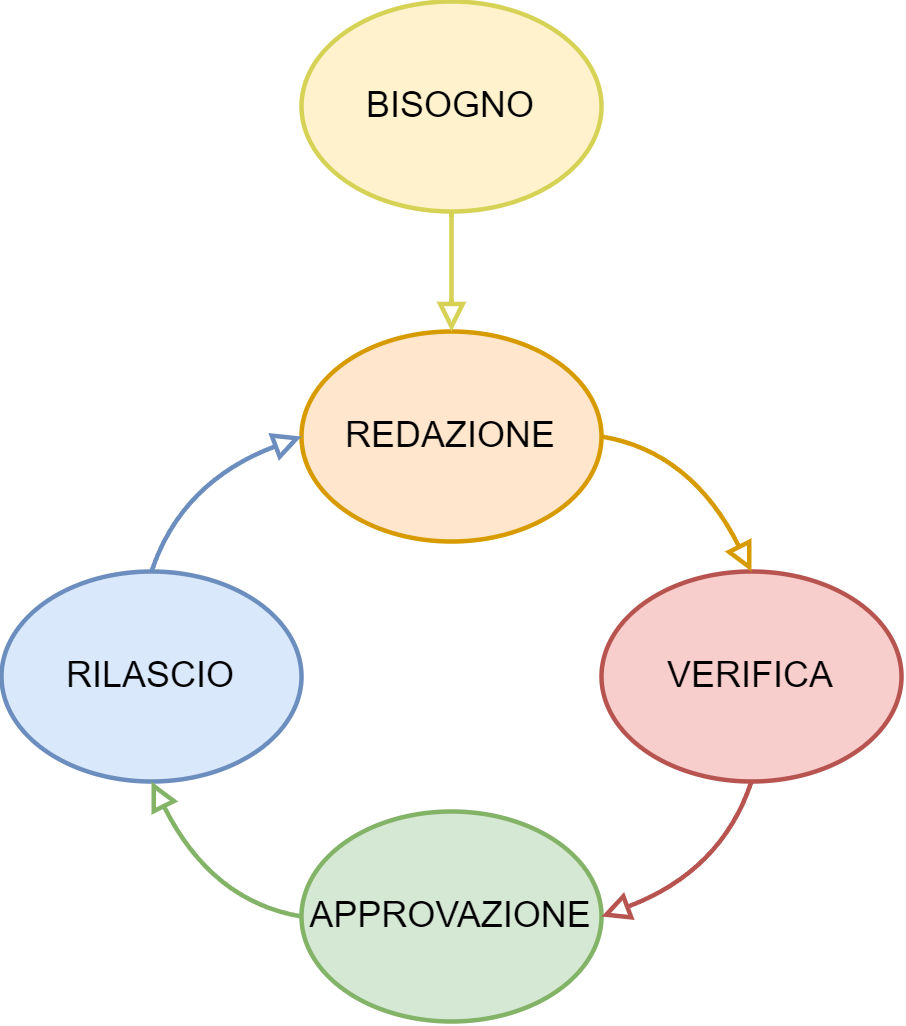
\includegraphics[scale=0.8]{doc_lifecycle.png}
    \caption{Ciclo di vita di un documento}
    \label{fig:doc_lifecycle}
\end{figure}

\subsubsection{Convenzioni adottate}\label{sec:processi_di_supporto:documentazione:convenzioni}
\paragraph{Nome del file}
Il nome del file deve seguire la convenzione snake case\textsuperscript{G}, ovvero:
\begin{itemize}
    \item Ciascuna parola è scritta completamente in minuscolo;
    \item Ogni parola è separata da un trattino basso `\_'.
\end{itemize}
Inoltre, ciascun documento deve riportare, alla fine del nome, il codice di versione.
\par Ad esempio, per il documento sulle norme di progetto di versione 0.0.1 il nome del file deve essere:
\begin{center}
    norme\_di\_progetto\_v0.0.1
\end{center}
\paragraph{Stile del testo}
\begin{itemize}
    \item \textbf{Grassetto}: utilizzato per i titoli delle sezioni e per i primi termini degli elenchi puntati oppure, se necessario, per evidenziare termini di maggiore importanza;
    \item \textbf{Corsivo}: utilizzato per citare il nome dei documenti (e.g. \textit{Analisi dei requisiti}).
\end{itemize}

\paragraph{Altre convenzioni}
\begin{itemize}
    \item Gli elenchi puntati devono rispettare le seguenti regole:
        \begin{itemize}
            \item Ogni elemento dell’elenco deve iniziare con la lettera maiuscola;
            \item Ogni elemento dell'elenco deve terminare o con ”;”, ad eccezione dell’ultimo elemento che deve terminare con ”.”. In caso di elementi particolarmente lunghi (e.g. composti da più frasi), si può decidere di utilizzare per tutti gli elementi il "." al posto di ";".
            \item Se gli elementi dell'elenco terminano con ";", in caso di sotto-elenchi, gli elementi di quest'ultimi termineranno con "," ad eccezione dell'ultimo elemento che deve terminare con ";" o "." a seconda di quanto discusso nel punto precedente.
        \end{itemize}
    \item Le immagini sono sono inserite sempre con una didascalia descrittiva posizionata sotto l’immagine. Il logo è l'unica immagine che fa da eccezione a questa regola.
    \item Le tabelle sono provviste di didascalia descrittiva posizionata sotto alla tabella. La tabella contenente il registro delle modifiche è l’unica che fa da eccezione a questa regola.
\end{itemize}


\subsubsection{Glossario}
All’interno della documentazione si possono trovare dei termini che possono risultare ambigui a seconda del contesto, o non conosciuti dagli utilizzatori.
Per ovviare ad incomprensioni si è deciso di stilare un elenco di termini di interesse accompagnati da una descrizione del loro significato. Questi termini sono riportati nel \textit{Glossario}.
Se il documento utilizza termini contenuti nel \textit{Glossario} di progetto, questi vanno segnalati nella sola prima istanza tramite la lettera \textbf{G} in apice, come da esempio:
\begin{center}
    termine\textsuperscript{G}
\end{center}
Inoltre, ogni componente del gruppo all’inserimento di un termine ritenuto ambiguo deve preoccuparsi di aggiornare il \textit{Glossario}.
\subsubsection{Struttura del documento}
Il gruppo ha scelto di utilizzare una struttura fissa e prestabilita per la documentazione, allo scopo di rendere più efficienti la stesura, la verifica e la comprensione, che sono tutte facilitate nel caso in cui lo schema di regole da seguire sia unico e preciso.
\paragraph{Struttura generica}
Questa sezione descrive la struttura di un documento qualsiasi prodotto nel corso del progetto, esclusi i verbali, che per loro natura hanno bisogno di una struttura diversa.
\par Un documento (non verbale) si compone di quattro parti, qui elencate nell'ordine in cui devono comparire sul documento, separate tra loro da interruzioni di pagina.
\subparagraph{Intestazione.}
L'intestazione ha una struttura verticale che deve contenere, nell'ordine di esposizione, centrati orizzontalmente:
\begin{itemize}
    \item Logo;
    \item Nome del gruppo;
    \item Email del gruppo;
    \item Titolo del documento;
    \item Informazioni sul documento;
    \begin{itemize}
        \item Versione;
        \item Nome e cognome del responsabile interno che ha approvato il documento;
        \item Nome e cognome di ciascun redattore;
        \item Nome e cognome di ciascun verificatore;
        \item Uso (interno o esterno).
    \end{itemize}
\end{itemize}
\subparagraph{Registro delle modifiche.}
Il registro delle modifiche descrive le modifiche apportate al documento nel corso del tempo, dalla prima scrittura a quella attuale. Il registro è riportato nel documento in forma tabellare: dove ogni riga rappresenta una modifica e contiene:
\begin{itemize}
    \item Versione del documento;
    \item Data di modifica;
    \item Autore della modifica;
    \item Ruolo dell'autore;
    \item Descrizione della modifica.
\end{itemize}
Le modifiche sono riportate, nell'ordine, dalla più vecchia alla più nuova.
\subparagraph{Indice dei contenuti.}
Questa sezione deve contenere un indice dei contenuti esposti nel documento, con i relativi numeri di pagina. Nel caso di documenti il cui contenuto è principalmente grafico (come l'analisi dei requisiti) o tabellare, sarà necessario inserire anche degli indici per le immagini o tabelle del documento.
\subparagraph{Argomenti.}
La sezione argomenti ha l'obiettivo di descrivere, gli argomenti discussi, le decisioni prese ed eventuali problematiche sorte nel corso dell'incontro. Per una comprensione più efficiente da parte del lettore, le descrizioni devono essere complete ma quanto più concise possibile.
%se è generale argomenti da scrivere più in generale e non per forza per un incontro?

%Questa sezione descrive la struttura di un documento qualsiasi prodotto nel corso del progetto, esclusi i verbali, che per loro natura hanno bisogno di una struttura diversa.
%aggiunta dell'elenco figure o tabelle
\paragraph{Struttura di un verbale}
La struttura di un verbale ha una sezione dedicata perché, vista la differenza di informazioni che deve contenere, possiede una sua particolare struttura, diversa dagli altri documenti.
\par Un verbale si compone di cinque parti, qui elencate nell'ordine in cui devono comparire sul documento, separate tra loro da interruzioni di pagina.
\subparagraph{Intestazione.}
L'intestazione ha una struttura verticale che deve contenere, nell'ordine di esposizione, centrati orizzontalmente:
\begin{itemize}
    \item Logo;
    \item Nome del gruppo;
    \item Email del gruppo;
    \item Titolo del documento;
    \item Sottotitolo con obiettivo dell'incontro (nel solo caso di un verbale esterno);
    \item Informazioni sul documento:
    \begin{itemize}
        \item Versione,
        \item Nome e cognome del responsabile interno che ha approvato il documento,
        \item Nome e cognome di ciascun redattore,
        \item Nome e cognome di ciascun verificatore,
        \item Uso (interno o esterno).
    \end{itemize}
\end{itemize}
\subparagraph{Registro delle modifiche e firma di approvazione.}
Il registro delle modifiche descrive le modifiche apportate al documento nel corso del tempo, dalla prima scrittura a quella attuale. Il registro è riportato nel documento in forma tabellare: dove ogni riga rappresenta una modifica e contiene:
\begin{itemize}
    \item Versione del documento;
    \item Data di modifica;
    \item Autore della modifica;
    \item Ruolo dell'autore;
    \item Descrizione della modifica.
\end{itemize}
Le modifiche sono riportate, nell'ordine, dalla più vecchia alla più nuova.
\par Nonostante il verbale sia un documento che, per sua natura, richiede meno modifiche rispetto agli altri (che hanno uno sviluppo più incrementale), il gruppo ha scelto di inserire un changelog per tenere traccia anche di eventuali richieste di modifica da parte dell'approvatore esterno prima della sua approvazione finale.
\par Alla fine del registro delle modifiche deve essere presente, nel solo caso dei verbali esterni, uno spazio per la firma di approvazione del partecipante esterno. Questa sezione deve contenere:
\begin{itemize}
    \item Versione del documento;
    \item Data della firma;
    \item Nome del firmatario;
    \item Spazio per la firma.
\end{itemize}
\subparagraph{Indice dei contenuti.}
Questa sezione deve contenere un indice dei contenuti esposti nelle due sezioni successive, con i relativi numeri di pagina.
\subparagraph{Informazioni.}
La sezione contiene le informazioni relative all'incontro descritto dal verbale. In particolare, deve riportare:
\begin{itemize}
    \item Informazioni di contesto:
    \begin{itemize}
        \item Modalità: in presenza o da remoto (eventualmente su quale piattaforma),
        \item Data dell'incontro,
        \item Orario di inizio e orario di fine;
    \end{itemize}
    \item Partecipanti:
    \begin{itemize}
        \item Interni, suddivisi tra presenti e assenti,
        \item Esterni.
    \end{itemize}
\end{itemize}
Se per l'incontro il gruppo ha selezionato un portavoce, questo deve essere segnato vicino al suo nome nell'elenco dei presenti.
\subparagraph{Argomenti.}
La sezione argomenti ha l'obiettivo di descrivere, gli argomenti discussi, le decisioni prese ed eventuali problematiche sorte nel corso dell'incontro. Per una comprensione più efficiente da parte del lettore, le descrizioni devono essere complete ma quanto più concise possibile.
\subsubsection{Template}
Al fine di mantenere una struttura quanto più coerente possibile e di velocizzare la scrittura della documentazione, il gruppo ha costruito un template per ciascun tipo di documento (verbale o generico), sul quale il redattore si deve basare per stilare un nuovo documento. Il template è disponibile come progetto dell'account Overleaf del gruppo.
\subsubsection{Strumenti}
\paragraph{\LaTeX}
Per la scrittura dei documenti il gruppo ha scelto di utilizzare \LaTeX, un linguaggio di marcatura creato appositamente per la preparazione di testi, basato sul programma per la tipografia digitale \TeX. Lo strumento facilita la stesura di un documento perché molti aspetti, quali ad esempio la numerazione delle sezioni, delle pagine e l'indice dei contenuti, vengono gestiti in maniera automatica, permettendo al redattore di focalizzarsi sul contenuto e lavorare in maniera più efficiente. Inoltre, è possibile lavorare su file diversi e unirli per costruire un singolo documento, facilitando la collaborazione tra membri del gruppo.
\par Lo strumento è reperibile al sito:
\begin{center}
    \url{https://www.latex-project.org/}\\ \textcolor{gray}{\textit{(ultimo accesso 10-04-24)}}
\end{center}
\paragraph{Visual Studio Code}
Visual Studio Code è un editor di codice sorgente libero, gratuito e leggero che permette, tramite l'utilizzo del plugin ``LaTeX workshop", un utilizzo veloce del linguaggio \LaTeX, fornendo strumenti come l'autocompletamento, la segnalazione di errori e la compilazione del documento in formato PDF.
\par Lo strumento è reperibile al sito:
\begin{center}
    \url{https://code.visualstudio.com/}\\ \textcolor{gray}{\textit{(ultimo accesso 10-04-24)}}
\end{center}
\paragraph{Diagrams.net}
Per la costruzione di diagrammi, in particolare per i diagrammi UML, il gruppo utilizza diagrams.net, una piattaforma gratuita per il disegno di grafi, che fornisce supporto a diverse tipologie di diagrammi, selezionata per la sua interfaccia semplice ed intuitiva e per la possibilità di salvare gli schemi prodotti in molti formati.
\par Lo strumento è reperibile al sito:
\begin{center}
    \url{https://www.drawio.com/}\\ \textcolor{gray}{\textit{(ultimo accesso 10-04-24)}}
\end{center}

\paragraph{JSDoc}
Per la scrittura dei commenti a supporto del codice del progetto si utilizza JSDoc, un linguaggio markup usato per la documentazione di codice Javasctipt. Si è scelto questo strumento data la sua compatibilità con Visual Studio Code, di cui sopra.
\par Lo strumento è reperibile al sito:
\begin{center}
    \url{https://jsdoc.app/}\\ \textcolor{gray}{\textit{(ultimo accesso 10-04-24)}}
\end{center}

\subsubsection{Metriche}\label{sec:processi_di_supporto:documentazione:metriche}
Per perseguire la qualità sulla documentazione prodotta si è deciso di adottare le seguenti metriche:
\begin{itemize}
    \item \textbf{MPC15-EOD}: Errori ortografici per documento;
    \item \textbf{MPC16-IG}: Indice Gulpease.
\end{itemize}
Per indicazioni più specifiche sulle suddette metriche si faccia riferimento al \textit{Piano di Qualifica}, presente tra i \hyperref[sec:riferimenti_esterni]{Riferimenti Esterni} del documento.

%%%%%%%%%%%%%%%%%%%%%%%%%%%%%%%%%%%
%%% GESTIONE DELLA CONFIGURAZIONE
%%%%%%%%%%%%%%%%%%%%%%%%%%%%%%%%%%%
\subsection{Gestione della configurazione}\label{sec:processi_di_supporto:gestione_configurazione}
La gestione della configurazione è l'attività dello sviluppo software che si occupa della gestione e controllo dei software items\textsuperscript{G}, in particolare della documentazione e del codice prodotto, nel corso del progetto.
\par È un processo particolarmente importante: permette di tracciare le modifiche nel tempo, migliora la collaborazione attraverso la condivisione dei file ed assicura una maggiore affidabilità del sistema, perché facilita l'individuazione e la risoluzione di errori.
\subsubsection{Versionamento}
Per poter identificare una particolare istanza di un software item in uno specifico momento temporale e differenziarla dalle altre, il gruppo ha scelto di assegnare un codice di versionamento a ciascun item che si preveda possa subire modifiche ed evolvere nel corso del progetto. Il codice utilizza cifre numeriche ed è scritto come segue:
\begin{center}
    \textbf{[X].[Y].[Z]}
\end{center}
Dove \textbf{X}, \textbf{Y} e \textbf{Z} sono numeri interi tali che:
\begin{itemize}
    \item \textbf{X}: è un numero $ \geq 0 $ che aumenta ad ogni approvazione del responsabile interno;
    \item \textbf{Y}: è un numero $ \geq 0 $ che aumenta ad ogni controllo del verificatore;
    \item \textbf{Z}: è un numero $ \geq 0 $ che aumenta ad ogni modifica del redattore;
    \item Se \textbf{Y} aumenta di 1, allora \textbf{Z} torna al valore 0;
    \item Se \textbf{X} aumenta di 1, allora sia \textbf{Y} che \textbf{Z} tornano al valore 0.
\end{itemize}
Ciascun software item inizia dalla versione \textbf{0.0.1} e prosegue come descritto.
\subsubsection{Strumenti}
\paragraph{Git}
Lo strumento principale utilizzato per questo processo è Git, un software per il controllo di versione con interfaccia a riga di comando. Si tratta di uno strumento molto famoso ed estremamente utilizzato, progettato per avere alte prestazioni e per garantire l'integrità dei file che gestisce: per queste ragioni, è considerato lo standard \textit{de facto} nell'ambito dei version control systems.
\par Lo strumento è reperibile al sito:
\begin{center}
    \url{https://git-scm.com/}\\ \textcolor{gray}{\textit{(ultimo accesso 10-04-24)}}
\end{center}
\paragraph{Gitflow}
Altra caratteristica importante di Git è la sua flessibilità di utilizzo: infatti, esistono diverse strategie di utilizzo per questo strumento, definite workflows, il cui obiettivo è stabilire delle linee guida per utilizzare Git in maniera consistente e produttiva.
\par Il workflow che il gruppo ha deciso di adottare è Gitflow, che suggerisce di assegnare ruoli specifici ai diversi branch e definisce le modalità secondo cui devono interagire.
\par Nello specifico, l'adozione del Gitflow workflow comporta la creazione di quattro tipologie di branch:
\begin{itemize}
    \item \textbf{Main}: è il ramo principale, sul quale si trova l'ultima versione funzionante e rilasciata del prodotto. Non si lavora mai direttamente sul ramo principale, per lasciarne intatto il contenuto.
    \item \textbf{Release}: è il ramo in cui si lavora per fare le ultime operazioni prima di un rilascio: una volta che tutto è pronto, il suo contenuto viene passato al main e rappresenta ufficialmente una nuova versione.
    \item \textbf{Develop}: è il ramo su cui si lavora principalmente, contiene il prodotto incompleto e in fase di lavorazione. Quando lo sviluppo raggiunge una fase tale per cui il prodotto è pronto per il rilascio, si passa il contenuto nel ramo release per gli ultimi ritocchi.
    \item \textbf{Feature}: ogni ramo feature si stacca dal develop e serve per lavorare separatamente su una specifica feature del prodotto (una parte di codice oppure un documento), in modo tale che il ramo develop non subisca alterazioni mentre la feature è in fase di lavorazione.
\end{itemize}
In particolare, un aspetto importante di questo workflow è la separazione dei lavori: infatti, permette a ciascun utente di lavorare sul progetto senza bloccare gli altri, perché si lavora su rami feature separati e, in ogni caso, non si lavora sul main, che quindi contiene sempre un prodotto funzionante e completo.
\par Maggiori informazioni sono presenti alla sezione \ref{sec:riferimenti_esterni:materiali_di_studio}, che contiene documentazione e tutorial sugli strumenti di progetto.


\subsection{Accertamento della qualità}\label{sec:processi_di_supporto:accertamento_qualità}
Lo scopo del processo di accertamento della qualità è quello di garantire che i processi e il prodotto siano conformi alle attese e soddisfino al meglio le richieste del proponente. 
A tal scopo, ogni membro del gruppo deve:
\begin{itemize}
    \item Comprendere le attività da svolgere e gli obiettivi da raggiungere;
    \item Aver compreso le metriche inserite nel documento di \textit{Piano di Qualifica} e rispettare le normative e gli standard definiti al suo interno;
    \item Mantenere le normative inserite nelle \textit{Norme di Progetto}.
\end{itemize}
Inoltre, vogliamo poter valutare il prodotto tramite verifiche retrospettive\textsuperscript{G}, effettuando confronti, in modo da poter osservare lo stato di avanzamento e l'andamento del progetto\textsuperscript{G} e perseguire un miglioramento continuo.
A tal fine e per avere una valutazione oggettiva e quantificabile della qualità, viene redatto il \textit{Piano di Qualifica}.

\subsubsection{Piano di qualifica}
Il \textit{Piano di Qualifica} 
%mettere link?
viene utilizzato come strumento per attuare gli obiettivi posti dal processo di accertamento della qualità tramite la:
\begin{itemize}
    \item Definizione dei requisiti del richiedente e, conseguentemente, degli obiettivi di qualità da perseguire;
    \item Definizione di un sistema di controllo della qualità che permetta di monitorare il livello delle prestazioni durante tutto il ciclo di vita del prodotto al fine di poter identificare le attività migliorabili;
    \item Definizione di metriche che misurino precisamente la qualità di ciascuna attività nell'ambito della verifica e della validazione;
    \item Definizione della quantità e tipologia dei test\textsuperscript{G} da effettuare per garantire la qualità del software;
    \item Visualizzazione di un cruscotto\textsuperscript{G} dello stato attuale, come sorta di resoconto delle attività di verifica\textsuperscript{G}.
\end{itemize}

\paragraph{Denominazione delle metriche}
Le metriche vengono identificate univocamente tramite un codice standardizzato dal gruppo nella seguente maniera:
\begin{center}
    \textbf{M[Tipo][Identificativo]-[Acronimo]}
\end{center}
dove:
\begin{itemize}
    \item \textbf{Tipo:} indica se la metrica misura la qualità di:
        \begin{itemize}
            \item \textbf{PC}: un processo;
            \item \textbf{PD}: un prodotto.
        \end{itemize}                 
    \item \textbf{Identificativo:} si tratta di un numero progressivo univoco all'interno di uno stesso \textit{Tipo}.
    \item \textbf{Acronimo:} indica l'acronimo del nome della metrica.
\end{itemize}
Inoltre, per ogni metrica viene riportata una breve descrizione e i valori accettabili e ottimali per avere un deliverable\textsuperscript{G} di qualità.

\paragraph{Denominazione dei test}\label{sec:processi_di_supporto:accertamento_qualità:test}
I test vengono identificati univocamente tramite un codice standardizzato dal gruppo nella seguente maniera:
\begin{center}
    \textbf{T[Tipo]-[Identificativo]}
\end{center}
dove:
\begin{itemize}
    \item \textbf{Tipo:} indica il tipo di test a cui si riferisce:
        \begin{itemize}
            \item \textbf{U}: test di unità;
            \item \textbf{I}: test di integrazione;
            %\item \textbf{R}: test di regressione;
            \item \textbf{S}: test di sistema;
            \item \textbf{A}: test di accettazione.
        \end{itemize}                 
    \item \textbf{Identificativo:} si tratta di un numero progressivo univoco all'interno di uno stesso \textit{Tipo} e strutturato in forma gerarchica \textit{[idPadre].[idFiglio]}. Viene usato per contraddistinguere i test e, se necessario, i loro sottocasi.
\end{itemize}
Inoltre, per ogni test viene riportata una breve descrizione e lo stato del test stesso. Quest'ultimo indicato come:
\begin{itemize}
    \item \textbf{NI}: se il test non è stato ancora implementato;
    \item \textbf{S}: se il test è stato implementato ed ha avuto esito positivo, i.e. test superato;
    \item \textbf{NS}: se il test è stato implementato ed ha avuto esito negativo, i.e. test non superato.
\end{itemize}
Si noti che un test avente dei ``figli'' viene considerato superato se e solo se tutti i suoi figli hanno avuto esito positivo.

%eventualmente aggiugere anche denominazione per test?
\subsubsection{Metriche}\label{sec:processi_di_supporto:accertamento_qualità:metriche}
Per tracciare la soddisfazione dei requisiti qualitativi è stata concordata una semplice metrica.
\begin{itemize}
    \item \textbf{MPC17-MS}: Metriche soddisfatte.
\end{itemize}
Per indicazioni più specifici sulla suddetta metrica si faccia riferimento al \textit{Piano di Qualifica}, presente tra i \hyperref[sec:riferimenti_esterni]{Riferimenti Esterni} del documento.


\subsection{Verifica}\label{sec:processi_di_supporto:verifica}
Il processo di verifica ha lo scopo di individuare, nella maniera più automatica possibile, gli errori commessi sia nella produzione del prodotto software sia nella produzione dei documenti, in modo che i deliverable\textsuperscript{G} siano completi e corretti e rispettino gli obiettivi di qualità definiti nel \textit{Piano di qualifica}.

Per ottenere tale risultato ci si affida ad attività di analisi e test svolti da programmatori e/o verificatori al termine di ogni fase di produzione. Tale analisi si differenzia in due diverse tipologie:
\begin{itemize}
    \item Analisi statica;
    \item Analisi dinamica.
\end{itemize}

\subsubsection{Analisi statica}
L'analisi statica consiste in una valutazione della forma, struttura e contenuto dell'oggetto da verificare e viene svolta prima che quest'ultimo venga eseguito. Pertanto, tramite questo tipo di analisi, possiamo verificare non soltanto il prodotto software o parti di esso, ma anche la documentazione.

Solitamente, questa particolare tipologia di valutazione si svolge tramite due metodi:
\begin{itemize}
    \item \textbf{Revisione (walkthrough):} lettura critica del codice usato per rivelare la presenza di difetti nell'oggetto da verificare, specie se non si sa con precisione dove questi potrebbero posizionarsi;
    \item \textbf{Ispezione (inspection):} lettura mirata dell’oggetto di verifica che focalizza la ricerca solo nei punti in cui è noto che potrebbero trovarsi delle problematiche.
\end{itemize}
Si noti che all'inizio il metodo di walkthrough avrà la prevalenza. Tuttavia, con l'avanzamento della produzione e il ripetersi del processo di verifica, sarà possibile sviluppare una ``Lista di Controllo''\textsuperscript{G} che contenga gli errori più comuni, consentendo un uso più intenso della tecnica di inspection, la quale risulta essere più efficiente.

\subsubsection{Analisi dinamica}
L'analisi dinamica, anche detta testing, consiste in una valutazione del comportamento in esecuzione dell'oggetto da verificare che, dunque, potrà essere solamente codice eseguibile.

In particolare, i test\textsuperscript{G} a cui sottoporre il software dovranno essere:
\begin{itemize}
    \item \textbf{Automatizzati:} si cerca di utilizzare degli strumenti che rendano il testing il più possibile automatizzato in modo da ottimizzare i tempi e ridurre l'errore umano;
    \item \textbf{Ripetibili:} si vuole poter ripetere un test più volte sullo stesso oggetto per poter verificare che le modifiche effettuate per risolvere le problematiche individuate siano effettivamente andate a buon fine.
\end{itemize}


\subsubsection{Strumenti}\label{sec:processi_di_supporto:verifica:strumenti}
\paragraph{Verifica della documentazione}
La verifica della documentazione consiste nel:
\begin{itemize}
    \item Lettura esplorativa del testo;
    \item Seconda lettura del testo per una migliore comprensione dei concetti esposti;
    \item Controllare, ed eventualmente segnalare, i concetti che risultano poco chiari, scorretti o non pertinenti;
    \item Controllare che la struttura del testo sia opportuna o suggerirne un'alternativa;
    \item Controllare, ed eventualmente segnalare, se il documento è completo o mancano delle parti;
    \item Controllare l'ortografia e la sintassi;
    \item Controllare, ed eventualmente segnalare, che a tutti i primi termini inseriti anche nel \textit{Glossario} sia stata inserita la lettera ``G'' in apice;
    \item Controllare che le convenzioni redazionali (stilistiche, tipografiche e strutturali) accordate nelle \textit{Norme di Progetto} siano state adottate.
\end{itemize}
A tal fine si utilizzano strumenti sia manuali che automatici:
\begin{itemize}
    \item \textbf{Controllo del verificatore:} il verificatore controlla completamente il documento alla ricerca di eventuali errori (metodo walkthrough);
    \item \textbf{Controllo dei punti della Lista di Controllo\textsuperscript{G}:} il verificatore controlla che l'oggetto da verificare non contenga nessun errore presente nella ``Lista di Controllo''\textsuperscript{G} (attività di inspection);
    \item \textbf{Plug-in degli editor:} si utilizzano dei plug-in offerti dagli editor di \LaTeX\space usati dal gruppo (Overleaf, VS-Code) per automatizzare il controllo della correttezza ortografica.
\end{itemize}

\paragraph{Verifica del codice}
Al fine di minimizzare gli errori, il codice viene controllato sia tramite analisi statica che dinamica. In particolare, si utilizzano i seguenti strumenti:
\begin{itemize}
    \item Per l'analisi statica: 
        \begin{itemize}
            \item \textbf{Controllo di verificatori e programmatori:} i programmatori e i verificatori durante le fasi di stesura e verifica ricercano eventuali problematiche. In particolare, controllano che i principi di buona programmazione siano stati rispettati ripercorrendo il codice e simulandone l'esecuzione.
        \end{itemize}
    \item Per l'analisi dinamica: 
        \begin{itemize}
            \item L’attività di analisi dinamica del codice si concretizza con lo sviluppo e l’utilizzo dei test. I test servono per assicurare un certo comportamento delle componenti oppure dell’intera applicazione. Ne esistono di diverse tipologie ed ognuna di queste va a controllare aspetti diversi del software (per maggiori informazioni si faccia riferimento al \textit{Piano di Qualifica}, presente tra i \hyperref[sec:riferimenti_esterni]{Riferimenti Esterni} del documento). In ogni caso, per ottenere un buon test, è necessario che questo sia ripetibile, oltre che specifichi ambiente di esecuzione, input e output. Pertanto, il gruppo intende utilizzare degli strumenti che automatizzino questa analisi, il gruppo ha definito Jest e React Testing Library come tali strumenti.
            %aggiungere tipo di test da effettuare per farli?
        \end{itemize}
\end{itemize}

\subsubsection{Metriche}\label{sec:processi_di_supporto:verifica:metriche}
Per mantenere la qualità nella verifica sono state scelte le seguenti metriche:
\begin{itemize}
    \item \textbf{MPC18-CCV}: Code coverage;
    \item \textbf{MPC19-TP}: Test passati.
\end{itemize}
Per indicazioni più specifiche sulle suddette metriche si faccia riferimento al \textit{Piano di Qualifica}, presente tra i \hyperref[sec:riferimenti_esterni]{Riferimenti Esterni} del documento.

\subsection{Validazione}\label{sec:processi_di_supporto:validazione}
Una volta terminata la fase di verifica, si può proseguire alla fase di validazione. Si noti che se la verifica viene effettuata in maniera corretta, anche quest'ultimo processo avrà un esito positivo.

Lo scopo della validazione è, infatti, quello di convalidare il prodotto sviluppato, confermando il soddisfacimento di tutti i requisiti concordati con il proponente (inseriti nel documento di \textit{Analisi dei requisiti})
% mettere link al documento?
e confermando il soddisfacimento delle aspettative dell'utente finale.
In particolare, sarà il responsabile del progetto che avrà la responsabilità di controllare i risultati decidendo se:
\begin{itemize}
    \item Accettare il prodotto in quanto conforme alle aspettative;
    \item Rifiutare il prodotto e richiedere una nuova verifica per correggere eventuali errori trascurati durante la precedente fase di verifica e/o per migliorare la qualità del prodotto.
\end{itemize}

\subsubsection{Metriche}\label{sec:processi_di_supporto:validazione:metriche}
Il processo di validazione non utilizza metriche qualitative particolari.

\newpage
%%%%%%%%%%%%%%%%%%%%%%%%%%%%%%%%%%%
% PROCESSI ORGANIZZATIVI
%%%%%%%%%%%%%%%%%%%%%%%%%%%%%%%%%%%
\section{Processi organizzativi}\label{sec:processi_organizzativi}
I processi organizzativi sono tutti quelli che riguardano l’organizzazione del gruppo e quindi definiscono funzioni e ruoli dei membri, oltre che metodi e regole da seguire per svolgere determinate operazioni.
Tutto ciò allo scopo di rendere il lavoro più efficace ed efficiente.
Essi si suddividono in attività di:
\begin{itemize}
    \item Gestione dei processi;
    \item Gestione delle infrastrutture.
\end{itemize}


\subsection{Gestione dei processi}\label{sec:processi_organizzativi:gestione_processi}
Questo processo riguarda le attività di carattere gestionale ed organizzativo che il gruppo deve svolgere per gestire gli altri processi nel corso del progetto. Sostanzialmente, descrive il coordinamento tra membri del gruppo e gli obiettivi che ciascuno deve raggiungere, così da poter monitorare spese e avanzamento del lavoro (e in particolare controllare il rispetto delle scadenze), oltre a poter quantificare i rischi.

Tutto ciò è raccolto nel \textit{Piano di progetto},
%link al file?
redatto dal responsabile, in collaborazione con l'amministratore. In particolare, esso espone:
\begin{itemize}
    \item Assegnazione dei ruoli e dei rispettivi compiti;
    \item Coordinamento, sia per quanto riguarda comunicazioni asincrone che tramite riunioni;
    \item Pianificazione e stima di tempi, risorse e costi;
    \item Valutazione dei rischi.
\end{itemize}

\subsubsection{Coordinamento}
Per il coordinamento durante l’intera durata del progetto il gruppo adotterà sia procedure di
\begin{itemize}
    \item \textbf{Comunicazione interna:} nel caso la comunicazione coinvolga solo i membri del gruppo;
    \item \textbf{Comunicazione esterna:} nel caso la comunicazione coinvolga anche proponente e/o committenti.
\end{itemize}
Nel caso la comunicazione avvenga sotto forma di riunione vengono redatti dai membri del gruppo (a rotazione) dei verbali degli incontri, approvati dal responsabile e, nel caso di comunicazione esterna, anche dal proponente/committente. Inoltre, prima di queste riunioni, il responsabile dovrà anche preparare una scaletta degli argomenti da trattare, che potranno essere poi integrati da eventuali dubbi e/o suggerimenti di altri membri del gruppo. 

\paragraph{Comunicazioni interne}
Le comunicazioni interne avvengono tramite le applicazioni:
\begin{itemize}
    \item \textbf{Telegram:} usato per la ``comunicazione veloce'' tra i membri del gruppo, sia di gruppo che individuale per comunicazioni più informali. In particolare, viene utilizzato per organizzare incontri interni e per brevi discussioni generali.
    \item \textbf{Discord:} usato come piattaforma per le riunioni del gruppo, attraverso il canale vocale, per discutere di temi che necessitano di un maggiore approfondimento.
\end{itemize}

\paragraph{Comunicazioni esterne}
Le comunicazioni esterne avvengono principalmente tramite le seguenti applicazioni:
\begin{itemize}
    \item \textbf{Gmail:} tramite l’indirizzo del gruppo \textit{sweavantgarde@gmail.com}.
    \item \textbf{Google Meet:} piattaforma di preferenza per le riunioni con il proponente.
\end{itemize}
Si noti che le comunicazioni esterne sono, in ogni caso, gestite dal responsabile di progetto. 

\subsubsection{Pianificazione}
\paragraph{Ruoli di progetto}\label{sec:processi_organizzativi:gestione_processi:pianificazione}
I ruoli vengono ruotati tra i membri del gruppo a cadenza periodica (generalmente ogni due settimane, ma cercando di garantire la continuità del lavoro), in modo da garantire che ogni membro assuma, nel corso del progetto, almeno una volta ogni ruolo e che lo assuma per un tempo congruo a quanto preventivato. 
Inoltre, si cerca di assegnare i ruoli in modo che non ci siano conflitti di interessi tra essi. Vige, infatti, la regola che un verificatore non può approvare il codice/testo che lui stesso ha scritto e, analogamente, un responsabile non può approvare il lavoro che lui stesso ha verificato. 

Sarà anche necessario tenere traccia delle ore che ogni componente dedica al progetto ed il ruolo associato a quelle ore, in modo da andare a rispettare la tabella degli impegni individuali. Per questo tracciamento verrà utilizzato un foglio Excel in cui ogni componente del gruppo segnerà le ore di lavoro settimanalmente.\\

\noindent Elenchiamo di seguito i ruoli previsti per il progetto e i rispettivi compiti.
\subparagraph{Responsabile.}
Il suo compito è quello di garantire il rispetto delle scadenze e di pianificare e coordinare lo svolgimento delle attività, assegnando i compiti agli altri membri del gruppo. Egli si occupa anche di approvare il rilascio dei deliverable\textsuperscript{G}.
Inoltre, rappresenta il tramite tra il gruppo e gli enti esterni, i.e. proponente e committente. Pertanto, è necessario che il responsabile rimanga sempre aggiornato sullo stato di progresso del progetto. Si noti che in ogni momento è presente un solo responsabile.

In particolare, le sue responsabilità sono:
\begin{itemize}
    \item Presentazione del \textit{Diario di Bordo} in aula;
    \item Redazione del \textit{Piano di progetto} %mettere link
    assieme all'amministratore per pianificare le milestones\textsuperscript{G};
    \item Redazione dei punti da discutere prima di ogni meeting interno del gruppo;
    \item Approvazione delle task verificate (su GitHub rilasciando le feature approvate sul branch main e, nello specifico per la documentazione, trasformando il codice \LaTeX\space in formato PDF);
    \item Gestione delle comunicazioni esterne.
\end{itemize}

\subparagraph{Amministratore.}
Il suo compito è quello di assicurare efficienza\textsuperscript{G} ed efficacia\textsuperscript{G} dei processi, in particolare per quanto riguarda la gestione degli strumenti e tecnologie che supportano il way of working\textsuperscript{G}. Anche in questo caso, in ogni momento è presente un solo amministratore.

Nello specifico si occupa di:
\begin{itemize}
    \item Redigere il documento \textit{Norme di Progetto};
    \item Redigere assieme al responsabile il \textit{Piano di Progetto};
    %mettere link?
    \item Redigere assieme ai progettisti il \textit{Piano di Qualifica};
    %mettere link?
    \item Gestire infrastruttura e strumenti utilizzati (e.g. gestire la board per l'organizzazione del lavoro), anche per quanto riguarda segnalazioni e problemi del gruppo riguardanti problemi e malfunzionamenti con gli stessi;
    \item Individuare i punti di miglioramento dei processi, ad esempio cercando modi per automatizzarli, valutando anche la possibilità di utilizzo di nuove tecnologie (facendo, in tal caso, uno studio preliminare in modo da poter presentare al gruppo pro e contro);
    \item Effettuare il controllo di versioni e configurazioni del prodotto software.
\end{itemize}

\subparagraph{Analista.}
Il suo compito consiste nello studiare a fondo il capitolato e le necessità/richieste del proponente allo scopo di individuare i requisiti fondamentali che il prodotto dovrà soddisfare. Chiaramente, per queste caratteristiche, questo ruolo è fondamentale nella prima parte del progetto\textsuperscript{G}.

In particolare, dunque, le sue mansioni sono:
\begin{itemize}
    \item Interrogare il proponente sullo scopo del prodotto e le funzionalità che lo stesso deve garantire;
    \item Studiare il problema, anche immedesimandosi in prima persona (testando tecnologie analoghe o similari già presenti in commercio) per comprendere a fondo le richieste del proponente e, in seguito, modellarne concettualmente un sistema risolutivo;
    \item Individuare i requisiti del progetto e suddividerli per categorie;
    \item Redigere il documento di \textit{Analisi dei requisiti}.
    %mettere link?
\end{itemize}

\subparagraph{Progettista.}
Il suo compito è quello di svolgere le attività di design, ovvero di progettare un'architettura\textsuperscript{G} che possa soddisfare i requisiti individuati dall'analista.

Nello specifico si occupa si:
\begin{itemize}
    \item Studiare l'architettura\textsuperscript{G} più adatta al prodotto, garantendone la qualità e il soddisfacimento dei requisiti;
    \item Scegliere eventuali pattern architetturali da implementare;
    \item Sviluppare lo schema UML delle classi;
    \item Individuare le unità architetturali\textsuperscript{G} che garantiscano la maggiore manutenibilità ed economicità, oltre che il minor numero di dipendenze possibili (i.e. con alto grado di coesione tra componenti ma basso grado di accoppiamento);
    \item Redigere la \textit{Specifica Tecnica} e la parte più pragmatica del \textit{Piano di Qualifica};
    \item Effettuare scelte per quanto riguarda gli aspetti tecnici e tecnologici del progetto.
    %mettere link?
\end{itemize}

\subparagraph{Programmatore.}
Il suo compito è implementare l'architettura prodotta dai progettisti.

Nello specifico le sue mansioni sono:
\begin{itemize}
    \item Scrivere codice, pulito e facile, seguendo le specifiche di progettazione (date dallo schema delle classi) e le regole definite nelle \textit{Norme di Progetto};
    \item Realizzare gli strumenti per la verifica e validazione del software, scrivendo gli eventuali test;
    \item Redigere il documento \textit{Manuale Utente}.
    %mettere link?
\end{itemize}
Si noti che in un primo momento del progetto\textsuperscript{G} il ruolo di ``Programmatore'' era stato sostituito dal ruolo di ``Redattore'' per la scrittura dei documenti di carattere generale (e.g. verbali).

\subparagraph{Verificatore.}
Il suo compito è controllare che le attività svolte dagli altri membri del gruppo siano prive di errori e rispettino la qualità prevista nel \textit{Piano di Qualifica} e le convenzioni definite nelle \textit{Norme di progetto}. %mettere link? 

In particolare, ha la responsabilità di:
\begin{itemize}
    \item Esaminare prodotti (sia software che di documentazione) in fase di revisione, tramite tecniche e strumenti definiti nelle \textit{Norme di Progetto}, verificando che requisiti funzionali e qualità siano rispettati;
    \item Segnalare eventuale errori e anomalie riscontrate in modo che possano essere corrette nel minor tempo possibile.
\end{itemize}

\paragraph{Metodo di lavoro e gestione delle task}\label{sec:pianificazione:gestione_task}
Per facilitare il corretto utilizzo delle procedure e degli strumenti, il gruppo deve delineare il proprio way of working\textsuperscript{G} e descriverlo formalmente in un documento, consultabile da ciascun membro in qualsiasi momento.  Il documento di riferimento è quello delle \textit{Norme di Progetto}, che deve essere redatto in maniera incrementale, aggiornando le procedure, le convenzioni e gli strumenti utilizzati durante il corso del progetto.

Inoltre, per una maggiore efficienza, si organizza il lavoro in task utili al raggiungimento di ogni milestone\textsuperscript{G} prefissata nel \textit{Piano di progetto} da responsabile e amministratore. %mettere link?
Lo scopo è quello di facilitare uno sviluppo autonomo del progetto, che consenta di rendere il lavoro il più possibile in parallelo e in asincrono.
Il compito di definire e predisporre le task viene svolto subito dopo la pianificazione della milestone\textsuperscript{G} attraverso l'uso di Github e seguendo il seguente iter:
\begin{itemize}
    \item \textbf{Creazione della task:} l'attività viene definita come compito da svolgere (\textit{TO-DO}) sotto forma di ticket direttamente su Github;
    \item \textbf{Assegnazione della task:} viene assegnata l'attività a seconda del ruolo corrente dei membri del gruppo;
    \item \textbf{Completamento:} l'attività viene completata da chi sta svolgendo il compito in quel momento, ma può essere ripresa in un secondo momento se necessario;
    \item \textbf{Verifica:} un verificatore controlla la task;
    \item \textbf{Accettazione:} a seguito della conferma del verificatore, il responsabile esegue un controllo e fa passare di stato l'attività decidendo se approvarla definitivamente o rifiutarla, richiedendo una nuova modifica/verifica.
\end{itemize}
Inoltre, per minimizzare ritardi e massimizzare lo svolgimento di queste task il gruppo ha deciso di dividere il tempo di lavoro in sprint, ossia dei piccoli intervalli all'interno di un periodo di circa due settimane (ridotti poi a intervalli di una settimana per il periodo seguente all'RTB) secondo il framework Agile Scrum.
In particolare, vengono identificate le seguenti fasi:
\begin{itemize}
    \item \textbf{Sprint Planning:} si fa un brainstorming sulle attività da svolgere durante il periodo di sprint, definendo quali task sono da completare a seconda di impegni e del preventivo orario dei membri da impiegare;
    \item \textbf{Sprint Review:} si svolgono delle riunioni di revisione in cui si commisurano i risultati ottenuti, dividendo gli obiettivi raggiunti da quelli non raggiunti;
    \item \textbf{Sprint Retrospective:} si conclude definitivamente lo sprint valutandone l'andamento e capendo le parti migliorabili e le parti che sono state fatte bene.
\end{itemize}

\subsubsection{Metriche}\label{sec:processi_organizzativi:gestione_processi:metriche}
Il processo di gestione dei processi non utilizza metriche qualitative particolari.


\subsection{Gestione delle infrastrutture}\label{sec:processi_organizzativi:gestione_infrastrutture}
Per la gestione dei processi organizzativi, i.e. per coordinamento e pianificazione, si rendono necessari degli strumenti che ne garantiscano l'efficacia e l'efficienza. Questi strumenti fanno parte della cosiddetta infrastruttura organizzativa.
Di seguito vengono riportati gli strumenti utilizzati.

\subsubsection{Strumenti}
%\paragraph{Jira}
%È un software che fornisce strumenti di pianificazione e monitoraggio permettendo ai team di progetto di avere una migliore organizzazione del lavoro. In particolare, consente la gestione delle issues\textsuperscript{G} che ciascun membro deve svolgere, permettendo l'assegnazione di attività a specifici membri e la definizione di dipendenze tra di esse.
%\par Lo strumento è reperibile al sito:
%\begin{center}
%    \url{https://www.atlassian.com/software/jira}
%\end{center}

\paragraph{GitHub}
Viene utilizzato come servizio di hosting della repository\textsuperscript{G}, quindi per archiviare e gestire il codice e tenere traccia delle modifiche e delle versioni. In particolare, per la gestione della repository viene utilizzato il workflow \textit{GitHub Flow} (maggiori informazioni su di esso sono presenti alla sezione \ref{sec:riferimenti_esterni:materiali_di_studio}).

A seguito della revisione RTB\textsuperscript{G}, viene anche utilizzato come strumento di pianificazione e monitoraggio del lavoro al posto di Jira. In particolare, si utilizzano le GitHub Issues\textsuperscript{G} per assegnare le attività ai specifici membri e definire dipendenze tra le stesse. Per ogni issue, inoltre, potranno essere assegnate anche alcune delle seguenti labels, secondo diversi criteri di interesse (come ambito o priorità):
\begin{itemize}
    \item \textbf{Da approvare}: indica una issue che necessita di approvazione;
    \item \textbf{Da verificare}: indica una issue che necessita di verifica;
    \item \textbf{Documentazione}: indica una issue riguardante la documentazione;
    \item \textbf{P=Bassa}: indica una issue a priorità bassa, con una scadenza di massimo 15 giorni;
    \item \textbf{P=Media}: indica una issue a priorità media, con una scadenza di massimo 7 giorni;
    \item \textbf{P=Alta}: indica una issue a priorità alta, con una scadenza di massimo 3 giorni.
\end{itemize}
Le issues vengono assegnate a delle milestones per verificarne il raggiungimento. La scadenza di ogni milestone viene discussa e fissata dal gruppo. 

\paragraph{Telegram}
Viene utilizzato come strumento di comunicazione interna asincrona, perlopiù per comunicazioni organizzative, grazie alla creazione di una chat condivisa con tutti i membri. Si utilizzano anche le chat individuali per questioni che interessano solo alcuni membri del gruppo.

\paragraph{Discord}
Viene utilizzato come strumento per la comunicazione sincrona interna al gruppo. In particolare, il server discord del gruppo è strutturato in due categorie di canali:
\begin{itemize}
    \item \textbf{Canale vocale:} canale principale di comunicazione per gli incontri interni;
    \item \textbf{Canale testuale:} canale utilizzato come supporto del canale vocale per la condivisione di risorse durante gli incontri.
\end{itemize}

\paragraph{Google Mail}
Si utilizza l’indirizzo e-mail condiviso \textit{sweavantgarde@gmail.com} per le comunicazioni esterne come gruppo con il proponente e il committente.

\paragraph{Google Meet}
Viene utilizzato come strumento di video-chiamata per le riunioni esterne con committente e proponente.

\subsubsection{Metriche}\label{sec:processi_organizzativi:gestione_infrastrutture:metriche}
Il processo di gestione delle infrastrutture non utilizza metriche qualitative particolari.

\subsection{Formazione del personale}\label{sec:processi_organizzativi:formazione_personale}
Lo sviluppo di un progetto dipende notevolmente dalle abilità e dalle conoscenze del team: se i componenti sanno utilizzare gli strumenti e conoscono l'argomento del progetto, allora saranno in grado di realizzare un prodotto di qualità, più efficace ed efficiente e con tempi di lavoro ridotti.
\subsubsection{Modalità di formazione}
La materia di interesse, la programmazione 3D, è un argomento che i membri del gruppo non hanno avuto modo di approfondire nel loro percorso formativo, così come gli strumenti adottati.
\par Per questi motivi, il gruppo si impegna a mantenere un processo di formazione autonoma ed individuale durante il corso del progetto e a definire una serie di procedure ed automatismi (dove possibile), allo scopo di lavorare sfruttando interamente le opportunità che gli strumenti offrono, per poter soddisfare pienamente le aspettative del committente e del proponente.
\par I materiali di studio suggeriti possono essere consultati nella sezione \ref{sec:riferimenti_esterni:materiali_di_studio}, che riporta i riferimenti esterni alla documentazione e tutorial per gli strumenti e le tecnologie utilizzati nel progetto.

\newpage
%%%%%%%%%%%%%%%%%%%%%%%%%%%%%%%%%%%
% STANDARD ISO/IEC 12207
%%%%%%%%%%%%%%%%%%%%%%%%%%%%%%%%%%%
\newpage
\section{Standard ISO/IEC 12207}\label{sec:standard_iso/iec_12207}
ISO/IEC 12207 è uno standard internazionale nato con l'obiettivo di diventare il riferimento primario per la gestione del ciclo di vita\textsuperscript{G} del software: in effetti, è il modello più utilizzato e conosciuto, perciò rappresenta una buona garanzia di successo se applicato correttamente nello sviluppo software.
\par Si tratta di uno standard più descrittivo che tecnico: infatti, riconosce la possibilità che il ciclo di sviluppo possa variare a seconda delle necessità e perciò non definisce un approccio specifico, ma piuttosto delinea una serie di processi che il ciclo deve attraversare, in una struttura modulare e flessibile per permettere agli utilizzatori di adattarlo alle proprie esigenze.
\par Lo standard suddivide i processi in tre categorie: processi \textbf{primari} (o \textbf{base}), processi di \textbf{supporto} e processi \textbf{organizzativi}, qui descritti in maniera sommaria per permettere al lettore una migliore comprensione della struttura del documento. Per una lettura più approfondita e rigorosa, si rimanda alla sezione \hyperref[sec:riferimenti_esterni]{Riferimenti Esterni}, che contiene un link alla versione originale (1995) dello standard.

%%%%%%%%%%%%%%%%%%%%%%%%%%%%%%%%%%%
%%% PROCESSI PRIMARI
%%%%%%%%%%%%%%%%%%%%%%%%%%%%%%%%%%%
\subsection{Processi primari}
Sono cinque processi a stretto contatto con lo sviluppo software che servono ai principali soggetti coinvolti nel suo ciclo di vita.
\subsubsection{Acquisizione}
Descrive le attività e gli obiettivi dell'acquirente, cioè di quel soggetto che identifica un'opportunità: ha il bisogno di acquisire un sistema, prodotto o servizio software, seleziona un fornitore e decide se accettare o meno tale sistema, prodotto o servizio proposto dal fornitore.
\par Le sottoattività in cui si suddivide questo processo sono infatti:
\begin{itemize}
    \item Acquisition preparation;
    \item Supplier selection;
    \item Supplier monitoring;
    \item Customer acceptance.
\end{itemize}
\subsubsection{Fornitura}
Questo processo, che delinea i compiti del fornitore, ha inizio nel momento in cui questo decide di produrre una proposta per rispondere alle richieste di un acquirente oppure quando firma un contratto con l'acquirente per lo sviluppo di un sistema, prodotto o servizio software. In particolare, il processo comprende la selezione di procedure e risorse necessarie a completare il progetto e la gestione dei rapporti con il cliente.
\par Il processo si suddivide nelle seguenti sottoattività:
\begin{itemize}
    \item Supplier tendering;
    \item Contract agreement;
    \item Product release;
    \item Product acceptance support.
\end{itemize}
\subsubsection{Sviluppo}
Contiene tutte le attività e gli obiettivi dello sviluppatore, dall'analisi dei requisiti, al design, alla programmazione con testing, fino all'installazione del prodotto, che deve soddisfare le richieste di contratto stipulate con il cliente.
\par Più nello specifico, il processo si suddivide in diverse sottoattività:
\begin{itemize}
    \item Requirements elicitation;
    \item System requirements analysis;
    \item System architectural design;
    \item Software requirements analysis;
    \item Software architectural design;
    \item Software detailed design;
    \item Software coding and testing;
    \item Software integration;
    \item Software qualification testing;
    \item System integration;
    \item System qualification testing;
    \item Software installation.
\end{itemize}
\subsubsection{Gestione operativa}
Il processo riguarda l'installazione ed erogazione del prodotto software, con riferimento anche al sistema nel quale il prodotto opera e al supporto per gli utenti utilizzatori.
\par Si suddivide in:
\begin{itemize}
    \item Operational use;
    \item Customer acceptance.
\end{itemize}
\subsubsection{Manutenzione}
Il processo si attiva quando il prodotto software deve essere modificato nel codice e di conseguenza nella documentazione associata, per risolvere difetti oppure per apportare miglioramenti o adattamenti a seconda delle necessità e ha come obiettivo quello di modificare il prodotto, mantenendo la sua integrità. Il processo include la migrazione e il ritiro del prodotto e, di fatto, si conclude proprio con quest'ultima fase.

%%%%%%%%%%%%%%%%%%%%%%%%%%%%%%%%%%%
%%% PROCESSI DI SUPPORTO
%%%%%%%%%%%%%%%%%%%%%%%%%%%%%%%%%%%
\subsection{Processi di supporto}
Sono otto processi, ciascuno con un suo obiettivo ben definito che, come il nome suggerisce, supportano altri processi e possono essere utilizzati da questi ogni volta che lo ritengano necessario.

\subsubsection{Documentazione}
Il processo di documentazione si occupa di registrare le informazioni prodotte dai processi durante il ciclo di vita del prodotto e delinea un elenco di attività che seguono la redazione di un documento nelle sue diverse fasi: dalla pianificazione e progettazione, alla scrittura e modifica, fino alla distribuzione e manutenzione.
\subsubsection{Gestione della configurazione}
Applica procedure tecniche e di amministrazione durante il ciclo di vita software con l'obiettivo di identificare i diversi software items, registrare il loro stato nel tempo e gestirne le modifiche ed i rilasci.
\subsubsection{Accertamento della qualità}
Si occupa di accertarsi che il software in produzione sia conforme agli specifici requisiti richiesti dal cliente e che rispetti i piani e gli standard prestabiliti. Può fare uso di altri processi di supporto, come verifica e validazione, revisione con il cliente, verifiche interne e risoluzione dei problemi.
\subsubsection{Verifica}
Ha l'obiettivo di determinare se le attività compiute durante il corso del progetto sono conformi alle specifiche decise nelle attività precedenti. Nella fase di sviluppo, ad esempio, la verifica spesso consiste nell'esecuzione ripetuta di test su porzioni più o meno grandi del codice (ma anche sul prodotto nella sua interezza) per capire se il programma si sta comportando in maniera coerente con quanto stabilito nella fase di design.
\par È consigliabile che questo processo abbia inizio quanto prima possibile nei processi primari che lo includono.
\subsubsection{Validazione}
La validazione ha il compito di accertarsi che le attività di progetto risultino in un prodotto finale che rispetti i requisiti preposti dal cliente e soddisfi i bisogni originali per i quali il progetto ha avuto origine.
\subsubsection{Revisione congiunta con il cliente}
Questo processo nasce per valutare assieme agli stakeholders lo stato e gli output delle diverse attività di progetto, per accertarsi che rispettino gli accordi prestabiliti e per decidere come intervenire in caso contrario.
\par Può essere impiegato sia a livello di gestione del progetto che a livello tecnico, preferibilmente durante tutto il corso del progetto.
\subsubsection{Verifiche ispettive interne}
Conosciuto anche come \textit{audit}, è un processo di revisione nel quale uno o più soggetti (detti \textit{auditors}) si accertano che il software sia conforme agli standard, ai requisiti e al contratto con il cliente.
\par Per tutelare il cliente ed ottenere una revisione imparziale, è necessario che gli auditors non siano direttamente responsabili del prodotto che stanno esaminando.
\subsubsection{Risoluzione dei problemi}
Ha lo scopo di analizzare e risolvere i problemi di qualunque natura che possono sorgere durante l'esecuzione di altri processi (in particolare, i processi di sviluppo, gestione operativa e manutenzione), con l'obiettivo di intervenire velocemente ed in maniera responsabile.
\par È importante anche documentare qualsiasi tipo di problematica per poterle poi classificare per categoria e per individuare certi tipi di pattern.

%%%%%%%%%%%%%%%%%%%%%%%%%%%%%%%%%%%
%%% PROCESSI ORGANIZZATIVI
%%%%%%%%%%%%%%%%%%%%%%%%%%%%%%%%%%%
\subsection{Processi organizzativi}
Sono quattro processi trasversali che non riguardano lo specifico progetto, ma l'aspetto di management e dovrebbero essere impiegati dall'organizzazione per migliorare la propria struttura e coordinazione.
\subsubsection{Gestione dei processi}
Contiene tutta una serie di obiettivi ed attività di carattere gestionale che possono essere impiegate da qualsiasi soggetto coinvolto per gestire i propri processi. In particolare, si suddividono in attività di:
\begin{itemize}
    \item \textbf{Pianificazione: }per ciascun processo, bisogna stabilire i lavori da svolgere, stimare il tempo necessario a concluderli, determinare le risorse necessarie e i costi, assegnare i ruoli e le responsabilità.
    \item \textbf{Esecuzione e controllo:} per mettere in atto il piano stabilito e monitorare l'andamento del processo, per assicurarsi che tutto proceda secondo i piani.
    \item \textbf{Revisione:} nella quale ci si assicura che il prodotto e i piani soddisfino i requisiti preposti, valutando anche l'andamento del processo rispetto alla pianificazione iniziale.
\end{itemize}
\subsubsection{Gestione delle infrastrutture}
Il processo ha il compito di stabilire e mantenere attiva l'infrastruttura necessaria per gli altri processi. Tale infrastruttura può essere di carattere sia software che hardware, ma può riguardare anche strumenti, tecniche e standard.
\subsubsection{Miglioramento del processo}
Si occupa di effettuare misure e controlli per stabilire e migliorare i processi di ciclo di vita del software.
\subsubsection{Formazione del personale}
Dato che la buona riuscita di tutti i processi (in particolare quelli primari) dipende dalle abilità e conoscenze del personale, questo processo si occupa di accertarsi che il personale abbia una formazione adeguata per i compiti che si trova a svolgere durante il corso del progetto.

\newpage
%%%%%%%%%%%%%%%%%%%%%%%%%%%%%%%%%%%
% RIFERIMENTI ESTERNI
%%%%%%%%%%%%%%%%%%%%%%%%%%%%%%%%%%%
\newpage
\section{Riferimenti esterni}\label{sec:riferimenti_esterni}
Per ulteriori chiarimenti sugli argomenti discussi nel documento, si possono consultare i seguenti link esterni:
\begin{itemize}
    \item \textbf{Glossario v1.0.0}:\\
    \url{https://github.com/Avant-Garde-Software-Engineering/WMS3D/blob/main/Documentazione/RTB/Esterna/glossario_v1.0.0.pdf}
    \item \textbf{Piano di Qualifica v2.0.0}:\\
    \url{https://github.com/Avant-Garde-Software-Engineering/WMS3D/blob/main/Documentazione/RTB/Esterna/piano_di_qualifica_v2.0.0.pdf}
    \item Capitolato \textbf{Warehouse Management 3D}:\\
    \url{https://www.math.unipd.it/~tullio/IS-1/2023/Progetto/C5.pdf} 
    \item \textbf{Regolamento} del progetto didattico:\\
    \url{https://www.math.unipd.it/~tullio/IS-1/2023/Dispense/PD2.pdf} 
    \item Link alla \textbf{documentazione del gruppo}:\\
    \url{https://avant-garde-software-engineering.github.io/documentazione.html} \textcolor{gray}{\textit{(ultimo accesso 10-04-24)}}
    \item Standard \textbf{ISO/IEC 12207}, versione 1995:\\
    \url{https://www.math.unipd.it/~tullio/IS-1/2009/Approfondimenti/ISO_12207-1995.pdf} 
    \item Link alle \textbf{slides sui processi del ciclo di vita}, con sottoattività per i processi dello standard ISO/IEC 12207:\\
    \url{https://www.math.unipd.it/~tullio/IS-1/2023/Dispense/T2.pdf} 
\end{itemize}
\subsection{Materiali di studio}\label{sec:riferimenti_esterni:materiali_di_studio}
\subsubsection{Documentazione}
\begin{itemize}
        \item \LaTeX: \url{https://www.latex-project.org/help/documentation/} \textcolor{gray}{\textit{(ultimo accesso 10-04-24)}}
        \item Visual Studio Code: \url{https://code.visualstudio.com/docs} \textcolor{gray}{\textit{(ultimo accesso 10-04-24)}}
        \item Diagrams.net: \url{https://www.drawio.com/doc/#get-started-with-diagramsnet} \textcolor{gray}{\textit{(ultimo accesso 10-04-24)}}
        \item Git: \url{https://git-scm.com/doc} \textcolor{gray}{\textit{(ultimo accesso 10-04-24)}}
        \item Github: \url{https://docs.github.com/en} \textcolor{gray}{\textit{(ultimo accesso 10-04-24)}}
        \item React.js: \url{https://react.dev/learn} \textcolor{gray}{\textit{(ultimo accesso 10-04-24)}}
        \item Next.js: \url{https://nextjs.org/docs} \textcolor{gray}{\textit{(ultimo accesso 10-04-24)}}
        \item Three.js: \url{https://threejs.org/docs/index.html#manual/en/introduction/Installation} \textcolor{gray}{\textit{(ultimo accesso 10-04-24)}}
        \item React Three Fiber: \url{https://docs.pmnd.rs/react-three-fiber/getting-started/introduction} \textcolor{gray}{\textit{(ultimo accesso 10-04-24)}}
        \item Zustand: \url{https://docs.pmnd.rs/zustand/getting-started/introduction} \textcolor{gray}{\textit{(ultimo accesso 10-04-24)}}
        \item Ant Design: \url{https://ant.design/docs/react/introduce} \textcolor{gray}{\textit{(ultimo accesso 20-04-24)}}
        \item Jest: \url{https://jestjs.io/docs/getting-started} \textcolor{gray}{\textit{(ultimo accesso 20-04-24)}}
        \item React Testing Library: \url{https://testing-library.com/docs/react-testing-library/intro/} \textcolor{gray}{\textit{(ultimo accesso 20-04-24)}}
    \end{itemize}
\subsubsection{Tutorial}
\begin{itemize}
        \item Gitflow:
            \begin{itemize}
                \item \url{https://www.atlassian.com/git/tutorials/comparing-workflows/gitflow-workflow} \textcolor{gray}{\textit{(ultimo accesso 10-04-24)}}
                \item \url{https://danielkummer.github.io/git-flow-cheatsheet/} \textcolor{gray}{\textit{(ultimo accesso 10-04-24)}}
            \end{itemize}       
                        
    \end{itemize}